 \documentclass{article}

\usepackage{graphicx}
\usepackage[toc,page]{appendix}

\usepackage[a4paper]{geometry}
\usepackage[english]{babel}
\usepackage[T1]{fontenc}
\usepackage{hyperref}
\usepackage{amstext,amsmath,amsfonts}
\usepackage{dcolumn,booktabs}
\usepackage{color}
\usepackage{subfigure}
\usepackage{amsthm}

\makeatletter
\def\maketitle{%
  \null
  \thispagestyle{empty}%
  \vfill
  \begin{center}\leavevmode
    \normalfont
    {\LARGE \@title\par}%
    \vskip 1cm
    {\Large \@author\par}%
    \vskip 1cm
    {\Large \@date\par}%
  \end{center}%
  \vfill
  \null
  \cleardoublepage
  }
\makeatother
\title{Bachelor thesis}

\author{Kees ter Brugge\\}
                
                
\date{\today}

\begin{document}
 \maketitle



\newpage
\section{introduction and abstract}

%frood and obstfeld try to explain the divergence between the fundamentals model and the true price by introducing an intrinsic bubble into the model. A non-linearity that explain over-reaction to new information about future dividends. They have to assume dividends to follow a random walk.
%Driffill and Sola however find evidence against dividends following a random walk and for dividends harboring a two-state markov switching regime. Now the effect of the intrinsic bubble is being minimized.
\newpage

\section{Stock price models}

An often used model to valuate assets is a simplified version of the model Lucas (1978) suggests. In this model, there are a large number of infinitely lived and identical agents. We assume these agents to be risk neutral. This gives us the following stochastic difference equation for equilibrium prices
\begin{eqnarray}
P_t = e^{-r} E_t(D_t + P_{t+1}) \label{standard}
\end{eqnarray}
where $P_t$ is the real stock price at the beginning of period $t$, $D_t $ are the real dividends per share paid over period $t$ and $E_t$ is the mathematical expectation conditioned on information available at the beginning of period $t$. $e^{-r}$ is the discount rate, where $r $ is the constant, continuous real rate of interest. 

Equation (\ref{standard}) has multiple solutions. A particular one is the present-value solution $P_t^{pv}$, which is obtained by iterating and using the law of iterated expectation:
\begin{eqnarray}
P_t^{pv} &=& e^{-r} E_t(D_t) +  e^{-r} E_t(P_{t+1}) = e^{-r} E_t(D_t) +  e^{-r}E_t(e^{-r} E_{t+1}(D_{t+1} + P_{t+2}))  \notag \\
&=& e^{-r} E_t(D_t) + e^{-2r} E_{t}(D_{t+1}) + e^{-2r}E_t(e^{-r} E_{t+2}(D_{t+2} + P_{t+3})) \notag \\
&=& e^{-r} E_t(D_t) + e^{-2r} E_{t}(D_{t+1}) + e^{-3r}E_t(D_{t+2}) + \cdots \notag \\
&=& \sum_{s=0}^{\infty}e^{-(s+1)r}E_t(D_{t+s}) \label{present-value}
\end{eqnarray}
if we assume
\begin{eqnarray}
\lim_{s\rightarrow \infty} e^{-rs}E_t(P_s) = 0 \label{transversality}
\end{eqnarray}
Condition (\ref{transversality})is known as the transversality condition and can be interpretated as assuming that the present value of an asset at time infinity is zero. This rules out the possibility of infinitely lived agents holding on to their stocks for infinity. The present-value solution equates a stock's price to its discounted expected future payments. We assume the continuously compounded growth rate of expected dividends to be smaller than $r$, so that the present-value solution does not diverge and therefore always exists.

Another group of solutions to (\ref{standard}) is obtained by adding a rational bubble component
\begin{eqnarray}
P_t = P_t^{pv} + B_t \label{sum}
\end{eqnarray}
where 
\begin{eqnarray}
B_t = e^{-r}E_t(B_{t+1}) \label{rational}
\end{eqnarray}
These solutions violate condition (\ref{transversality})
unless the bubble component is equal to zero. Condition (\ref{rational}) excludes arbitrage oppurtunities.

\subsection{Intrinsic bubbles}
Froot and Obstfeld (1991) claim that the component of prices left unexplained by the present-value model is highly positively correlated with dividends. They suggest an 'intrinsic' bubble that only depends on fundamentals and not on extraneous factors. To find the function of this bubble, assumptions about the stochastic process for dividends $D_t$ have to be made. A common assumption is that log dividends $d_t$ are a random walk \footnotemark with constant drift $\mu$
\footnotetext{Froot and Obstfeld (1991) argue that a random walk is a plausible approximation to the mechanism the market uses to forecast dividends (see appendix A, p. 1209)}
\begin{eqnarray}
d_{t+1} = \mu + d_t + \xi_{t+1} \label{lognormal}
\end{eqnarray}
where $\xi_{t+1}$ is a normal random variable with conditional mean zero and variance $\sigma^2$. If we additionally assume $D_t$ to be known at the beginning of period $t$ and 
\begin{eqnarray}
P_t^{pv} &=&  \sum_{s=0}^{\infty}e^{-(s+1)r}E_t(D_{t+s}) = \sum_{s=0}^{\infty}e^{-(s+1)r}E_t(e^{d_{t+s}}) = \sum_{s=0}^{\infty}e^{-(s+1)r}E_t(e^{d_t + s\mu + \sum_{i=1}^{s} \xi_{t+i}}) \notag \\
 &=& D_t e^{-r} \sum_{s=0}^{\infty} e^{-sr + s\mu + \frac{s\sigma^2}{2}} = D_t e^{-r} \sum_{s=0}^{\infty} \left(e^{-r + \mu + \frac{\sigma^2}{2}}\right)^s
 = D_t e^{-r} \frac{1}{1 - e^{-r + \mu + \frac{\sigma^2}{2}}} \notag \\ 
 &=& D_t \frac{1}{e^r - e^{\mu + \frac{\sigma^2}{2}}} = D_t \kappa \label{kappa}
\end{eqnarray}
since $E_t(e^{\xi_{t+1}}) = e^{\frac{\sigma^2}{2}}$.  $\kappa$ represents the inverse of the required rate of return on stocks less the expected rate of growth of dividends and is equal to the ratio of the present-value price and dividends. It is defined as follows
\begin{eqnarray}
$\kappa = \frac{1}{e^r - e^{\mu + \frac{\sigma^2}{2}}}$ \label{eqkappa}
\end{eqnarray}
 The sum in (\ref{kappa})converges because we have assumed $r > \mu + \frac{\sigma^2}{2}$ to ensure the existence of the present-value solution.

The bubble proposed by Froot and Obstfeld is a nonlinear function of current dividends
\begin{eqnarray}
B(D_t) = cD_t^\lambda \label{intrinsic}
\end{eqnarray}
which satisfies condition (\ref{rational}) if the following condition holds
\begin{eqnarray}
\lambda = \frac{\sqrt{\mu^2 + 2r\sigma^2} - \mu}{\sigma^2} \label{eqlambda}
\end{eqnarray}
because then
\begin{eqnarray}
e^{-r}E_t(B(D_{t+1})) &=& e^{-r}E_t(cD_{t+1}^{\lambda}) = e^{-r}E_t(ce^{d_{t+1}\lambda}) = e^{-r}E_t(ce^{(\mu + d_t + \xi_{t + 1})\lambda}) \notag \\ 
 &=&  ce^{d_t\lambda}e^{-r + \lambda \mu }E_t(e^{\xi_{t+1}\lambda} = cD_t^{\lambda}e^{-r + \lambda \mu + \frac{\lambda^2 \sigma^2}{2}} = cD_t^{\lambda} = B(D_t) \notag
\end{eqnarray}
 We choose $\lambda$ to be the positive root of the equation, because we want the size of the bubble to go to zero as dividends go to zero. This implies $\lambda > 1$. $c$ is a nonnegative constant, because stock prices cannot be negative. It would violate free disposability.
Now we can rewrite (\ref{sum}) so that it includes an intrinsic bubble, obtaining our intrinsic bubble model.
\begin{eqnarray}
P_t = P_t^{pv} + B(D_t) = \kappa D_t + c D_t^{\lambda} \label{sumintrinsic}
\end{eqnarray}
When $\lambda$ is near to one this model can suffer from colinearity. Therefore it is better to use the price-dividend ratio model 
\begin{eqnarray}
\frac{P_t}{D_t} =  \kappa  + c D_t^{\lambda - 1} \label{sumratio}
\end{eqnarray}
While the present-value solution suggests a constant price-dividend ratio $\kappa$, the inclusion of an intrinsic bubble implies that the ratio is a function of dividends. 




\subsection{Nonlinear least squares data fitting}
If we want to estimate coefficients of a model with a nonlinear specification, we use the method of nonlinear least squares (NLS) estimation. We consider the nonlinear specification 

\begin{eqnarray}
y = f(\mathbf{x};\theta) + e(\theta) 
\end{eqnarray}
where $y$ is the dependent variable, $f$ a nonlinear function,  $\mathbf{x}\in \mathbb{R}^k$ a vector of explanatory variables, $\theta \in \mathbb{R}^l$ a vector of parameters and $e$ the specification error. Given T observation of $(y,\mathbf{x})$, let


\begin{eqnarray}
\textbf{y} = 
\begin{bmatrix}
y_1 \\ y_2 \\ \vdots \\ y _T \\ 
\end{bmatrix} \text{  ,  } 
f(\mathbf{X}; \theta) = 
\begin{bmatrix} 
f(\mathbf{x_1};\theta) \\
f(\mathbf{x_2};\theta) \\
\vdots \\
f(\mathbf{x_T};\theta) \\
\end{bmatrix} \text{  ,  }
\mathbf{e(\theta)} = 
\begin{bmatrix}
e_1(\theta) \\ e_2(\theta) \\ \vdots \\ e_T(\theta)
\end{bmatrix} 
\end{eqnarray}

We want to find the parameter $\theta$ for our function that best fits the data $(\mathbf{y,X})$. How well our choice of parameters is, is measured by the following formula
\begin{eqnarray}
 S(\theta) = [y - f(\mathbf{X};\theta]'[y - f(\mathbf{X};\theta]  \label{min}
\end{eqnarray}
We want to minimize $S(\theta)$ with respect to $\theta$. A solution $\theta^* \in \mathbb{R}^l$ to this problem must satisfy the first and second order condition of the minimization problem. The first order condition is that the the gradient of (\ref{min}) evaluated at $\theta^*$ must be equal to zero
\begin{eqnarray} 
\frac{dS(\theta)}{d\theta}(\theta^*) = -2 \frac{df(\mathbf{X};\theta)}{d\theta}(\theta^*) [y - f(\mathbf{X};\theta^*]
=  \mathbf{0} \label{foc}
\end{eqnarray}
where 
\begin{eqnarray}
\frac{df(\mathbf{X};\theta)}{d\theta}= 
\begin{bmatrix}
\frac{df(\mathbf{x_1};\theta)}{d\theta} & \frac{df(\mathbf{x_2};\theta)}{d\theta} & \cdots & \frac{df(\mathbf{x_T};\theta)}{d\theta}  \\
\end{bmatrix}
\notag
\end{eqnarray}

Furthermore, to ensure that $S(\theta^*)$ is a minimum and not a maximum, the second order condition of a minimization problem has to be satisfied. The hessian matrix of (\ref{min}), denoted below, evaluated at point $\theta^*$ must be a positive definite matrix.
\begin{eqnarray}   
\frac{d^2S(\theta)}{d\theta d\theta'} =  -2 \frac{d^2f(\mathbf{X};\theta)}{d\theta d\theta'} \cdot [y - f(\mathbf{X};\theta] + 2 \frac{df(\mathbf{X};\theta)}{d\theta} \cdot \frac{df(\mathbf{X};\theta)}{d\theta'} 
 \label{soc}
\end{eqnarray}

The problem with $f$ being nonlinear is that there can be multiple $\theta \in \mathbb{R}$ that satisfy these two conditions. If $f$ were linear, (\ref{foc}) would be a system with l equations and l unknowns. This would give us a unique solution. Furthermore, $\frac{d^2f(\mathbf{X};\theta)}{d\theta d\theta'} $ would be equal to zero and thus $\frac{d^2S(\theta)}{d\theta d\theta'} =  2 \frac{df(\mathbf{X};\theta)}{d\theta} \cdot \frac{df(\mathbf{X};\theta)}{d\theta'} $. This is a sufficient condition for positive definitness.  There is no garantee that there exists a unique solution to this problem if $f$ is nonlinear. This means (\ref{min}) can have multiple local minima. We cannot solve this problem analytically, but we can with an iterative process.
\\
There are a lot of iterative procedures that can lead to a fairly good approximation of the optimal parameter choice. An often used method is the Newton-Raphson algorithm. It uses the second order Taylor expansion of (\ref{min}) around some chosen initial value $\theta_0$
\begin{eqnarray}
S(\theta) \approx S(\theta_0) + (\frac{dS(\theta)}{d\theta}(\theta_0))' (\theta - \theta_0) + \frac{1}{2} (\theta - \theta_0)'\frac{d^2 S(\theta)}{d\theta d\theta'}(\theta_0)(\theta - \theta_0) \label{taylor}
\end{eqnarray}

The first order condition of this expansion with respect to $(\theta)$ is

\begin{eqnarray}
\frac{dS(\theta)}{d\theta}(\theta_0) + \frac{d^2 S(\theta)}{d\theta d\theta'}(\theta_0)(\theta - \theta_0) = 0 \notag
\end{eqnarray}
This can be rewritten as
\begin{eqnarray}
\theta = \theta_0 - (\frac{d^2 S(\theta)}{d\theta d\theta'}(\theta_0))^{-1} \frac{dS(\theta)}{d\theta}(\theta_0)
\end{eqnarray}
So we now know the value $\theta$ that minimizes the taylor expansion . If we now replace $\theta_0$ and $\theta$ with $\theta_i$ and $\theta_{i+1}$ respectively, we get the following algorithm
\begin{eqnarray}
\theta_{i+1} = \theta_i - (\frac{d^2 S(\theta)}{d\theta d\theta'}(\theta_i))^{-1} \frac{dS(\theta)}{d\theta}(\theta_i) \label{algorithm}
\end{eqnarray}
The $(i+1)^{th}$ iterated value $\theta_{i+1}$ is obtained from the value of the previous iteration. 
The downside of this algorithm is that for every iteration the hessian matrix must be positive definite, otherwise it might not be invertible of point in the wrong direction. From (\ref{taylor})(\ref{algorithm}) we can deduce that 
\begin{eqnarray}
S(\theta_{i+1}) - S(\theta_i)\approx   -\frac{1}{2}  (\frac{dS(\theta)}{d\theta}(\theta_i))'  \frac{d^2 S(\theta)}{d\theta d\theta'}(\theta_i)\frac{dS(\theta)}{d\theta}(\theta_i)
\end{eqnarray}
Succesive iterations of $S$ only become smaller if the hessian matrix is positive definite.\\
Sometimes a step length s is added to (\ref{min})
\begin{eqnarray}
\theta_{i+1} = \theta_i - s_i(\frac{d^2 S(\theta)}{d\theta d\theta'}(\theta_i))^{-1} \frac{dS(\theta)}{d\theta}(\theta_i)
\end{eqnarray}
The step length could be determined by minimizing $S(\theta_{i+1})$ with respect to $s_i$. 
\\
An iterative algorithm needs a beginning and an end. The beginning may be some initial value set of values. To minimize the risk of no iteration converging to the global minimum we can generate a lot of  initial values from some distribution and choose the initial value that gives the best result. An algorithm stops when some sort of convergence criteria is met. For example, when 
\begin{eqnarray}
(\theta{i+1} - \theta_i)'(\theta{i+1} - \theta_i) < c
\end{eqnarray}
where $c$ is some small positive pre-determined number. 








\newpage
\section{Application to Standard \&Poor's 500}


\begin{figure}[h!]
	\centering
		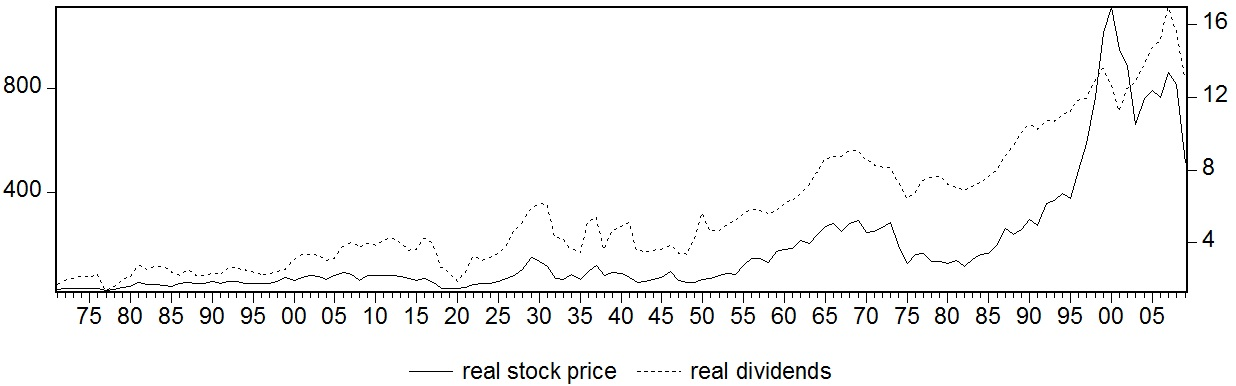
\includegraphics[width=0.99\textwidth]{C:/Users/kc/Downloads/divandprice.jpg}
	\caption{Plot of real dividends $D_t$ and real prices $P_t$ over 1871 - 2009. The left axis scales the prices and the right axis scales the dividends.}
	\label{pricediv}
\end{figure}

%decribe, plot data, show linear when logtransformed and stationary when differenced hence integrated order one.
To examine the validity of the models we defined before, we use data on the U.S. stock market from 1871 untill 2009. The used stockprice index is the January values of the Standard and Poor's Composite annual stock price index. The time series is an updated version of the often used data from Shiller (1989). Shiller used data till 1988, which gives us a oppurtunity to see if recent events, such as the dot-com bubble, change the results of the analysis of this model. Since data on January values of the dividends index are not available, we use annual averages for the calendar year, following Froot and Obstfeld (1991). They found that this does not affect results statistically\footnotemark. Stock prices and dividends are deflated by the Produces Price Index of 1982. \footnotetext{see Froot and Obstfeld (1991) footnote 18, p. 1198} We use data till 2006 to estimate the coefficients, so that we can perform out of sample forecasts to compare with the last three realizations. 
The Standard and Poor's composite index is considered as one of the best benchmarks of U.S. stock market performance. It is a market value weighted index that includes 500 stocks that trade on either the New York Stock Exchange and the NASDAQ. The selection of stocks is mostly based on market size, liquidity and sector. The S$\&$P monthly index series was created in 1957 and is extended back to January 1871 by Cowles. 
\

In figure (\ref{pricediv}) we see that dividends and prices seem to have an exponential trend. To assess the nature of these processes, we want to produce stationary series. In figure (\ref{logpricediv}) the log transformation of both series is shown. The series seem to have a linear trend now. The series move together, which indicates correlation of the series. Furthermore, their trend also seems equally steep, which suggests that these processes might be cointegrated.


\begin{figure}[t!]
	\centering	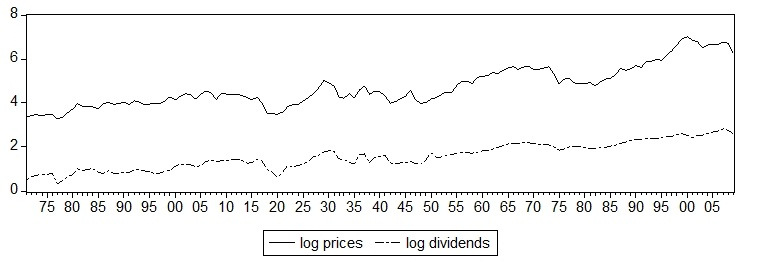
\includegraphics[width=0.99\textwidth]{C:/Users/kc/Downloads/logpricediv.jpg}
	\caption{Plot of log prices and log dividends over 1871 - 2009}
	\label{logpricediv}
\end{figure}

In figure (\ref{dlnpricediv}) the first difference of the log transformation of prices and dividends is plotted. The series appear to be stationary. This suggests $d_t$ and $p_t$ are integrated of order one. It is common to assume that a series is integrated of order one, when its log transformation  is integrated of order one. 

\begin{figure}[h!]
	\centering
		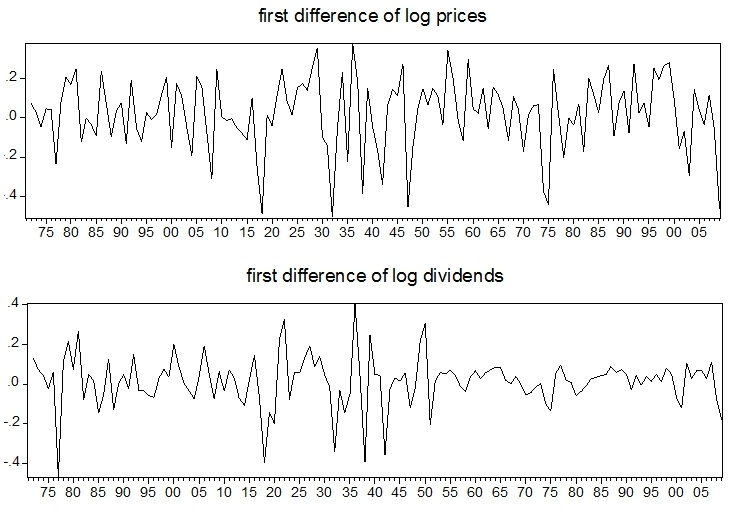
\includegraphics[width=0.99\textwidth]{C:/Users/kc/Downloads/dlogdivprice.jpg}
	\caption{Plot of $\Delta d_t$ and $\Delta p_t$ over 1872 - 2009}
	\label{dlnpricediv}
\end{figure}

If we look at figure (\ref{dlnpricediv}) we see that after 1955 $\Delta d_t$ becomes much less volatile. Since dividends is the explanatory variable of our model it is a good idea to analyse a subsample with 1955 as start date in addition to the whole sample.	 This could give us better estimates, which in turn leads to a better assessment of the statistical significance of the model and more accurate forecasts.  
\newpage
	
To be able to execute some tests on the intrinsic bubble model we have to assume that the error  term $\eta_t$ we add to (\ref{sumratio}) to get
\begin{eqnarray}
\frac{P_t}{D_t} =  c_0  + c D_t^{\lambda - 1} + \eta_t \label{intrinsicmodel}
\end{eqnarray}
is well-behaved, meaning that $\eta_t$ is statistically independent of dividends at all leads and lags and has unconditional mean zero\footnotemark. Otherwise the statistical tools we use do not lead to unbiased estimates. $\eta_t$ can be interpreted as any shock to the price-dividend ratio that has no predictive power with respect to future dividens, such as fads. 
%hier regressie van eta op epsilonsss
\footnotetext{Froot and Obstfeld (1991) also made these assumptions. For a justification see footnote 16, p. 1198}

Our null hypothesis is that there is no bubble, that the present-value model is true, so that the level of dividends has no impact one the price-dividend ratio  and therefore $c_0 = \kappa$ and $c=0$. Our alternative hypothesis is that there is a bubble involved, a relation between dividends and the price-dividend ratio, implying $c_0 = \kappa$ and $c > 0$. 


To obtain the estimates of $\kappa$ and $\lambda$ implied by the intrinsic bubble model, which we from now on denote as $\overline{\kappa}$ and $\overline{\lambda}$ respectively, we first have to obtain the point estimates of $\mu, \sigma$ and $r$. The estimates are reported in table (\ref{point}). We obtain the continuous interest rate as follows  $\overline{r} = log(\frac{\sum_{t=m}^{2005}\frac{P_{t+1} + D_t}{P_t}}{2005-m})$, where $m$ is $1871$ for the estimate based one the whole sample and  $1955$ based on the subsample. In figure (\ref{lnpricediv}) we clearly see that log dividends has a positive trend. Under the assumption that log dividends has no trend, the p-value of the estimate of $\mu$ is equal to 0.14 for the whole sample and 0.01 for the subsample.  $\overline{\kappa}$ and $\overline{\lambda}$ are obtained by using the point estimates in equation (\ref{eqkappa}) and (\ref{eqlambda}) respectively.


\begin{table}[h!]
\centering
\begin{tabular}{l | l l  }
\hline \\
parameter & whole sample 1871 - 2006 & subsample 1955 - 2006\\ \hline 
$r$  & 0.0904 & 0.1009 \\
$\mu$ & 0.0162 & 0.0204\\
$\sigma$ & 0.1257 & 0.0544 \\
$\kappa$ & 14.2411 & 11.8984 \\
${\lambda}$ & 2.5094 &  3.8634 \\
\end{tabular}
\caption{Estimates of parameters for the two samples}
\label{point}
\end{table}
The model estimates the coefficient $\lambda$ that indicates the explosiveness of the bubble much higher for the subsample than for the whole sample. 


\subsection{Present-value model}
The present-value model (\ref{present-value}) predicts that the following regression 
\begin{eqnarray}
$P_t = \beta_0 + \beta D_t  + v_t$ \label{regpv}
\end{eqnarray}
gives us an estimate of $\beta$ that is close to $\overline{\kappa}$. When we perform an regression on the log transformations of prices and dividends instead 
\begin{eqnarray}
$p_t = \beta_0 + \beta d_t  + v_t$ \label{reglnpv}
\end{eqnarray}
we expect to find an estimate of $\beta$ near one, since the linear relation between prices and dividends implied by the present-value model has an elasticity equal to one. \\

On the other hand, if (\ref{intrinsicmodel}) is true, the estimate of $\beta$ we expect to find from (\ref{regpv})  is much bigger than $\overline{\kappa}$, since the derivative of prices with respect to dividends predicted by the intrinsic model adds a positive nonlinear component to the derivative predicted by the present-value model
$$\frac{d P_t}{d D_t} = c_0 + \lambda c D_t^{\lambda - 1} >  c_0 = \frac{d P_t^{pv}}{d D_t}$$ 
Furthermore, (\ref{intrinsicmodel}) implies a nonlinear relation between $P_t$ and $D_t$ and since $\lambda$ is bigger than one, this relation has an explosive nature. The estimate of $\beta$ that follows from (\ref{reglnpv}) the log transformation of the variables should be bigger than one. Prices would appear to overreact to changes in dividends. 
\
\begin{table}[h!]
\centering
\begin{tabular}{l | l | l l l l }
\hline \\
regression equation & $\beta$ whole sample & $\beta$ subsample \\
\hline \\
 $P_t = \beta_0 + \beta D_t  + v_t$ &  56.0023 & 89.2800 \\
$p_t = \beta_0 + \beta d_t  + v_t$ & 1.4475 & 2.1273   \\ \hline 
\end{tabular}
\caption{OLS regression of real prices on a constant and real dividends.}
\label{sensitivity}
\end{table}

In table (\ref{sensitivity}) we see that the estimates of $\beta$ obtained by (\ref{regpv}) are much higher for both samples than the values in table (\ref{point}) predicted by the present-value model.  Furthermore, the coefficients obtained from (\ref{reglnpv}) are also much higher than the value predicted by the present-value model, one.

\begin{figure}
	\centering
		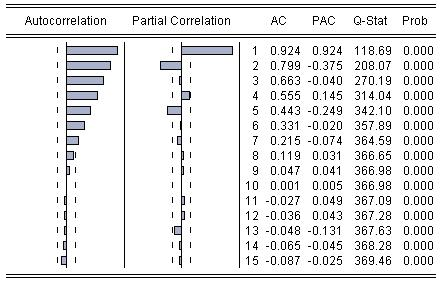
\includegraphics[width=0.99\textwidth]{C:/Users/kc/Downloads/1871pvcorrelo.JPG}
	\caption{correlogram of $v_t$ resulting from regression $P_t = \beta_0 + \beta D_t  + v_t$. Sample is 1871 - 2006. }
	\label{correlo}
\end{figure}

In figure (\ref{correlo}) we see the correlogram resulting from (\ref{regpv}) when the whole sample is used. The results are similar to those obtained by using only the subsample. The residuals are positively autocorrelated, so this model is not able to produce white noise residuals.  




Another way to assess the validity of the present-value model is to test for cointegration. Cointegration indicates a long-run relationship between two or more series. As can seen in figure (\ref{dlnpricediv}) log prices and log dividends seem to be integrated of order one. The phillips-Perron unit root test with intercept gives us the adjusted t-staticstics -0.64 and  -0.68 for the whole sample and -1.13 and -0.55 for the subsample respectively. The null hypothesis that log prices and log dividends are integrated of order one is not rejected. We assume prices and dividends are integrated of order one too. Under the present-value model various measures of the price-dividend ratio should produce stationary residuals.

\begin{table}[h!]
\centering
\begin{tabular}{l | l  }
\hline \\
Variables used in test for cointegration & whole sample & subsample \\
\hline \\
$P_t$ and D_t & 11.7263 & 11.6657 \\ 
$p_t$ and $d_t$ & 7.6584 & 6.8591  \\
\hline 
\end{tabular}
\caption{The reported values are the unrestricted cointegration rank test trace statistics obtained by the Johansen methodology under the null hypothesis of no cointegration, where * denotes statistical significance at the 5 \% level.

estimates of $\beta_1$ in the regression $\Delta x_{t+1} = \beta_0 + \beta_1 x_t + v_{t+1} $. The sample is 1871 - 2006. In parentheses under the estimates the Phillips-Perron test statistics are reported, where * denotes statistical significance at the 5 \% level.}
\label{cointegrationpv}
\end{table}



 test if prices and dividends are cointegrated. We test if there exists an equilibrium relationship to which these series eventually return. 


 any linear combination of dividends that moves together with prices in the long run. We check if prices and  

So we check if prices and dividends are cointegrated. our forecasted 
Finding that two processes are cointegrated is usefull, since you know that they cannot 
wander off in opposite directions for very long without coming back to a mean 
distance eventually.

If two processes seem to move together in the long run, they might be cointegrated

appear to always come back to some equilibrium relation,

 have a long-run relationship, it is usefull to test if they are cointegrated. Finding that two processes are cointegrated increases forecasting powers. If two time series are integrated of some order and a linear combination of these processes yields a time series that is integrated of a lower order, these time series are cointegrated. Prices and dividends are generally thought of as processes which are integrated of order one. If they are, then under the present-value model we would expect to find that a linear function, with cointegrating coefficient $\kappa$, of prices and dividends gives us a stationary time series. This linear function is called the spread by Campbell and Shiller's (1987). Equivalently, if we use the log prices and log dividends instead, we expect to find cointegration with cointegrating coefficient one. The price-dividend ratio is also expected to be stationary. Under (\ref{intrinsicmodel})  we expect the null hypothesises of nonstationarity of these various measures of the price-dividend ratio to not be rejected. 


\begin{table}[h!]
\centering
\begin{tabular}{l | l l }
\hline \\
Variable $X_t$ & $\beta_1$ with trend & $\beta_1$ without trend \\
\hline \\
$P_t $ & -0.0573 & -0.0214 \\
 & (-2.27) & (-1.27)\\
$p_t $ & -0.0871 & -0.0176  \\
 & (-2.58)  & (-1.09)\\
$D_t$ & -0.0757 & -0.0043 \\
 & (-2.34) & (-0.06) \\
$d_t$ & -0.2084 & -0.0233 \\
 & (-4.10)* & (-1.01) \\
$P_t - \overline{\kappa} D_t$ & -0.0619 & -0.0318 \\
 & (-2.40) & (-1.65) \\
$\frac{P_t}{D_t}$ & -0.0802 &  -0.0488 \\
 & (-2.65)& (-1.80) \\
$p_t - d_t$ &-0.1027 & -0.0590 \\
 & (-2.72)& (-1.93)\\
\hline 
\end{tabular}
\caption{The reported values are the estimates of $\beta_1$ in the regression $\Delta x_{t+1} = \beta_0 + \beta_1 x_t + v_{t+1} $. The sample is 1871 - 2006. In parentheses under the estimates the Phillips-Perron test statistics are reported, where * denotes statistical significance at the 5 \% level.}
\label{cointegrationpv}
\end{table}
%zeg wat over kracht en geloofwaardigheid van deze test.
As we can see in table (\ref{cointegrationpv}) seven out of eight tests do not reject the hypothesis that prices, dividends or their log transformations contain a unit root and are therefore nonstationary. Furthermore, for none of the measures of the price-dividend ratio was the null hypothesis of a unit root rejected. They were not able to produce a series that had a lower order of integration.  
\\

There are a few problems with the present-value model. It can not explain the high price-dividend ratios given the rate of return $\overline{r}$, prices are much more sensitive to dividends than predicted by the present-value model. When we test for a linear long-run relationship between prices and dividends, which under the present-value model should exist, we do not find evidence to support this relationship.  \\
 Furthermore, the result of the  regression of log prices on log dividends can be interpreted as evidence that the relation between prices and dividends is a nonlinear one.  









\subsection{Intrinsic bubble model}
To see if a nonlinear function of dividends describes the variation in price-dividend ratios more accurately than the present-value model, we estimate (\ref{intrinsicmodel}). To test for absence of an intrinsic bubble we first have to know the distribution of the t statistic under the null hypothesis. So, additional assumptions about the error term $\eta_t$ have to be made. Besides $\eta_t$ being identically distributed, independent of dividends at all leads and lags and having unconditional mean zero, we also assume that they have a normal distribution. The nonnegativity of price-dividend ratios is not likely to give any problems since the mean of the price-dividend ratios is more than three times the standard error of $\eta_t$. Even though (\ref{intrinsicmodel}) contains the explosive regressor $D_t^{\lambda - 1}$, the standard t statistic approximates a normal distribution under these assumptions\footnotemark. \footnotetext{see Froot and Obstfeld (1991), Appendix B}
\\
Since we have not assumed that $\eta_t$ is distributed independently, the residuals may be serially correlated. This can lead to incorrect estimations of the standard errors of coefficients. To counteract this, we correct the residuals using Newey and West's (1987) covariance matrix estimator.


\begin{table}[h!]
\centering
\begin{tabular}{l | l l l l l l}
\hline \\
estimated model & $ \widehat{c_0} $ & $ \widehat{c} $ & $\widehat{\lambda}$ &  F stat.$(c = 0)$ & $R^2$ & d.f. \\
\hline \\
$ \frac{P_t}{D_t} =  c_0  + c D_t^{\lambda - 1} + \eta_t $ & 16.8904 & 0.1824 & 3.0152 & 131.72 ** & 0.66 & 136\\
 & (8.06)** & (0.69) & (5.43)** & & &\\
$  \frac{P_t}{D_t} =  c_0  + c D_t^{\overline{\lambda} - 1} + \eta_t $ & 14.2736 & 0.6863 & & & 0.65 & 137  \\
 & (9.58)**  & (5.25)** & & & &\\
$ \frac{P_t}{D_t} =  \overline{\kappa}  + c D_t^{\lambda - 1} + \eta_t $ &  & 0.4284 & 2.7120 & 39113.20 ** & 0.65 & 137\\
 &  & (1.93)* & (7.19)** & & &\\
$  \frac{P_t}{D_t} =  \overline{\kappa}  + c D_t^{\overline{\lambda} - 1} + \eta_t $ &  & 0.6770 & & & 0.65 & 138  \\
 &   & (7.14)** & & & &\\
\hline 
\end{tabular}
\caption{nonlinear OLS regression. Sample is 1871 - 2009. Standard errors are corrected by the Newey-West covariance matrix, allowing for fourth-order serial correlation and conditional heteroskedasticity. In parentheses under the
estimates the standart t test statistics are reported, where *(**) denotes statistical significance at the 10(1)\% level.}
\label{regressionnonlinear}
\end{table}

In table (\ref{regressionnonlinear}) the results of the estimation of (\ref{intrinsicmodel}) are reported. The model is estimated with and without the restriction that $\lambda$ and $\kappa$ are equal to their point estimates obtained earlier from the log dividend process and the mean return on stock. When we restrict $\lambda = \overline{\lambda}$, the bubble coefficient $\widehat{c}$ is statistically very significant. When we do not restrict the exponent $\lambda $, $\widehat{c}$ gets smaller and $\widehat{\lambda}$ is estimated larger than its point estimate. The bubble coefficient becomes statistically insignificant. To test whether the nonlinear component is statistically insignificant, We use a F-test. We test  the restricted no bubble model where $c=0$ and $\lambda = \widehat{\lambda}$ versus the alternative bubble model where $ c \neq 0$ and  $ \lambda = \widehat{\lambda}$. The no bubble model is rejected at the 1\% level\footnotemark. \footnotetext{The F statistic is defined as follows: $F = \frac{RSS_1 - RSS_2}{p_2 - p_1} \cdot \frac{n - p_2}{RSS_2}$ where $RSS_1$, $p_1$, $RSS_2$ and $p_2$ denote the residual sum of squares and the amount of parameters of model 1 and 2 respectively. $n$ is the sample size.} We can use this test, since the no bubble model is nested in the bubble model. The estimates of $\kappa$ are almost equal to $\overline{\kappa}$. If we apply the restriction $\kappa = \overline{\kappa}$, $\widehat{\lambda}$ is almost equal to $\overline{\lambda}$.
\\
Another way to check the validity of the intrinsic bubble model is by testing for cointegration. Under (\ref{intrinsicmodel}) there should exist a long-run relationship between the variation in the price-dividend ratio left unexplained by the present-value model and the nonlinearly transformed dividend series. To assess if such a relation exists, we have to perform a nonlinear cointegration test. We use the method desribed by Granger and Hallman (1991).
We test if a linear combination of $\frac{P_t}{D_t} - \overline{\kappa}$ and the nonlinearly transformated dividends series $D_t^{\lambda - 1}$ can produce a series with a lower order of integration. The result are reported in table (\ref{cointegrationintrinsic}). The cointegration coefficient are obtained from table (\ref{regressionnonlinear})



\begin{table}[h!]
\centering
\begin{tabular}{l | l l }
\hline \\
Variable $X_t$ & $\beta_1$ with trend & $\beta_1$ without trend \\
\hline \\
$\frac{P_t}{D_t} - \overline{\kappa} - 0.4284 D_t^{1.7120} $ & -0.1620 & -0.1556 \\
 & (-3.94)* & (-3.84)**\\
$\frac{P_t}{D_t} - \overline{\kappa} - 0.6770 D_t^{\overline{\lambda} - 1} $ & -0.1536 & -0.1501  \\
 & (-3.82)*  & (-3.78)**\\
\hline 
\end{tabular}
\caption{The reported values are the estimates of $\beta_1$ in the regression $\Delta x_{t+1} = \beta_0 + \beta_1 x_t + \beta_2 t + v_{t+1} $ where $\beta_2$ is equal to zero in the regression without trend. The sample is 1871 - 2009. In parentheses under the estimates the Phillips-Perron test statistics are reported, where *(**) denotes statistical significance at the 5(1) \% level.}
\label{cointegrationintrinsic}
\end{table}

The results of a Phillips-Perron unit root test on the price-dividend ratio and on dividends are reported in table \ref{cointegrationpv}. For both these series, the unit root hypothesis cannot be rejected. For the sake of robustness we test with and without time trend, with and without restricting $\lambda$ for a unit root in variable $X_t$. In table (\ref{cointegrationintrinsic}) we see that in all four tests the unit root hypothesis is rejected. This means that the price-dividend ratio and the nonlinear transformation $D_t^{\lambda}$ are cointegrated. 
\\


\begin{figure}[b!]
	\centering
		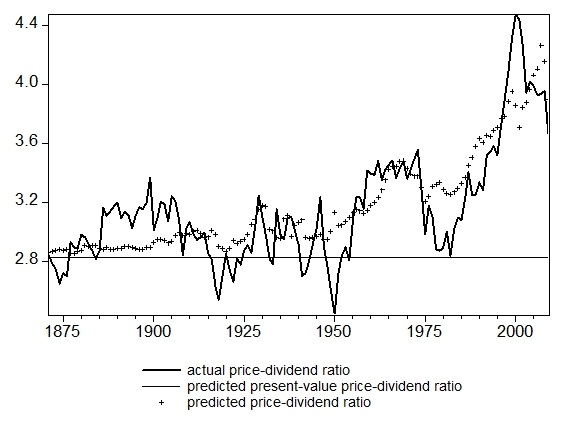
\includegraphics[width=0.99\textwidth]{C:/Users/kc/Downloads/ratiographs.jpg}
	\caption{This figure shows the log transformation of the following ratios: the actual price-dividend ratio $\frac{P_t}{D_t}$, the predicted price-dividend ratio under the intrinsic bubble model $\frac{\widehat{P}_t}{D_t} = \widehat{c}_0 + \widehat{c}D_t^{\widehat{\lambda} - 1}$ and its predicted present-value price-dividend ratio $\frac{\widehat{P}_t^{pv}}{D_t} = \widehat{c}_0$.
	The coefficients that are used are from the unrestricted regression found in table (\ref{regressionnonlinear}).}
	\label{ratiographs}
\end{figure}

The estimation of model (\ref{intrinsicmodel}) confirmed the explosive nature and the statistical significance of the bubble component in stock prices. The bubble component absorbs almost all the oversensitivity of prices to dividends, because when we include a nonlinear regressor in the regression, the estimates of $\kappa$ are close to its point estimate. This means model (\ref{intrinsicmodel}) does a good job of explaining the price-dividend ratio given the rate of return $\overline{r}$. This can also be seen in figure (\ref{ratiographs}). The positive correlation between the price-dividend ratio and the nonlinear bubble component implies that as dividends grow, the overvaluation of prices relative to the present-value price, grows exponentially. This is hardly noticable when dividends are low, but when dividends increase, prices explode. In figure (\ref{pricegraphs}) the size of the bubble component in prices can be estimated by comparing the stock price with the present-value price. Figure (\ref{pricegraphs}) and (\ref{ratiographs}) show that after the 1950's the economic relevance of the bubble component in stock prices and price-dividend ratios has grown. The nonlinear cointegration test showed us (\ref{intrinsicmodel}) produces stationary residuals, which means that in the long-run we have found a fairly good approximation of the underlying data generating process.





\begin{figure}[t!]
	\centering
		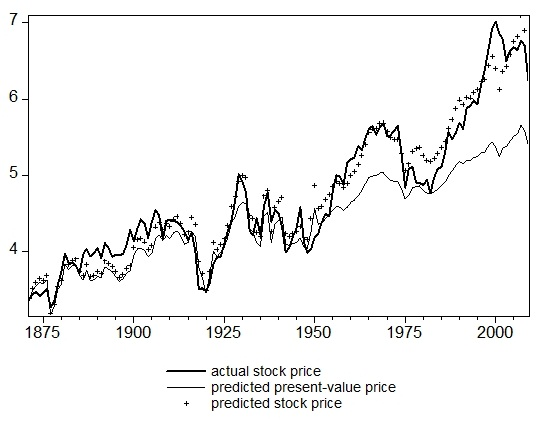
\includegraphics[width=0.99\textwidth]{C:/Users/kc/Downloads/pricegraphs3.jpg}
	\caption{This figure shows the log transformation of the following prices: the actual stock price $P_t$, the predicted stock price under the intrinsic bubble model $\widehat{P}_t = \widehat{c}_0D_t + \widehat{c}D_t^{\widehat{\lambda}}$ and its predicted present-value stock price $\widehat{P}_t^{pv} = \widehat{c}_0 D_t$.
	The coefficients that are use are from the unrestricted regression found in table (\ref{regressionnonlinear}).}
	\label{pricegraphs}
\end{figure}

\newpage

%add forecast static for 1880 with sample from 1950 and 1871. compare mean squared error, better yet plot them together with forecasts.

\section{Conclusion}
\section{References}
\end{document}







To allow for errors our model we generalize (\ref{sumintrinsic}) by adding a error term
  
To test our models we need estimates of $\mu, \sigma, r, \kappa$ and $\lambda $. The data on dividends estimates $\overline{\mu} = 0,0148 ,\overline{\sigma} = 0,1259$ and $r$ is estimated as follows
\begin{eqnarray}
\overline{r} = log(\frac{\sum_{t=1871}^{2009}\frac{P_{t+1} + D_t}{P_t}}{2009-1871}) = 0.0877 \label{r}
\end{eqnarray}
These point estimates give us $ \overline{\kappa} =14,5613 , \overline{\lambda}= 2,5214$. 
\subsection{price-dividend relation}
Under the present value model  a stock's price is a linear function of its dividends. 
\begin{eqnarray}
P_t^{pv} = \kappa D_t + u_t \label{pvmodel}
\end{eqnarray}
If this model holds in the long run, we expect to find prices and dividends to be cointegrated. Furthermore we expect the estimated value of $\kappa$ to be close to $\overline{\kappa}$. 

In figure 1 a plot of the stock price-dividends ratio is provided.  




\begin{figure}[h!]
	\centering
		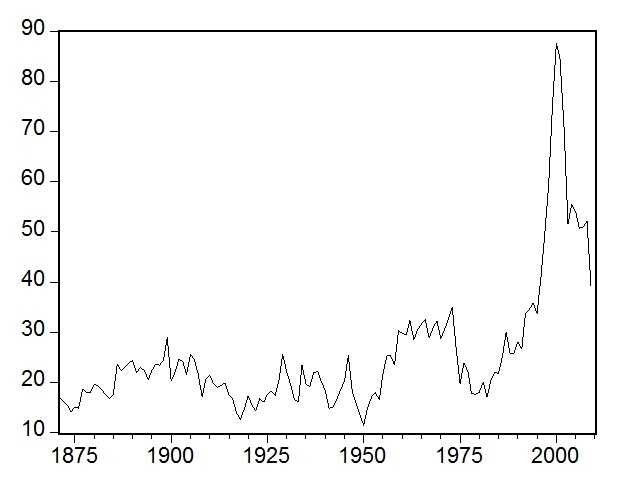
\includegraphics[width=0.85\textwidth]{C:/Users/kc/Downloads/ratio.jpg}
	\caption{price-dividend ratio 1871-2009}
	\label{fig:ratio}
\end{figure}


Using the Dickey-fulller test 


The intrinsic bubble model claims that a stock's price is nonlinear function of dividends. 


 check if price minus present value price is cointegrated with the nonlinearly transformed dividends series.



$\overline{r} = log(\frac{\sum_{t=1871}^{2009}\frac{P_{t+1} + D_t}{P_t}}{2009-1871} = 0.0877, \overline{\mu} = 0,0148 ,\overline{\sigma} = 0,1259 $, \\ $ \overline{\kappa} = \frac{1}{e^{\overline{r}}- e^{\overline{\mu} + \frac{1}{2}{\overline{\sigma}}^2}} = 14,5613 , \overline{\lambda}= 2,5214$

\section{conclusion}

\section{references}

\end{document}




\subsection{regime-swithching}

If any financial time series is being followed for sufficiently long, one is bound to see changes in behaviour. 
In time series where variables seem to display different types of behaviour, modelling this data as a markov-switching time series can be beneficial. Cecchetti, Lang and Mark (1990) and Bonomo and Garcia (1994) argue that there are regime-switches in dividends. Lets make the same assumptions as Driffill and Sola (1998); log dividends are a two-state Markov process
\begin{eqnarray}
d_{t+1} = dt + \mu_0(1 - s_{t+1}) + \mu_1 s_{t+1} + (\sigma_0 (1 - s{t+1}) + \sigma_1 s_{t+1})\epsilon_{t+1} 
\end{eqnarray}



%tot hier



pricing model with nonlinear more sensitive to new dividends and does better job at explaining over-reaction.


It models the over-reaction of 

 to current dividends. 

%van hier wordt t intrinsic bubbles.
We assume the expected growth of dividend payments to be lower than $e^{-r}$ to ensure the existence of this solution. Solution (\ref{fundamental}) is derived by applying the transversality condition.
\begin{eqnarray}
\lim_{s\rightarrow \infty} e^{-rs}E_t(P_s) = 0 
\end{eqnarray}
Another solution of (\ref{standard}) is the market fundamental solution plus a bubble component $B_t$.
\begin{eqnarray}
P_t = P_t^f + B_t
\end{eqnarray}
This can only be a solution of (\ref{standard}) if
\begin{eqnarray}
B_t = e^{-r}E_t(B_{t+1})
\end{eqnarray}
Bubbles which satisfy condition (\ref{rational}) are rational, there are no arbitrage oppurtunities.\\
Bubbles can be

Froot and Obstfeld (1991) suggest a type of bubble which only depends nonlinearly on dividend payments. A bubble that is a function of fundamental factors only is called an intrinsic bubble. To investigate these bubbles we have to specify the distribution of real dividends. We assume the log of real of real dividends, denoted by $d_t$, to be a random walk with drift $\mu$: 
\begin{eqnarray}
d_{t+1} = \mu + d_t + \xi_{t+1}  \\
d_{t+s} = d_t + s\mu + \sum_{i=1}^{s} \xi_{t+i}
\end{eqnarray}
where $\sum_{i=1}^{s} \xi_{t+i} \sim N(0,s\sigma^2)$. We assume $D_t$ to be known at the beginning of period $t$.
\begin{eqnarray}
P_t^f &=&  \sum_{s=0}^{\infty}e^{-(s+1)r}E_t(D_{t+s}) = \sum_{s=0}^{\infty}e^{-(s+1)r}E_t(e^{d_{t+s}}) = \sum_{s=0}^{\infty}e^{-(s+1)r}E_t(e^{d_t + s\mu + \sum_{i=1}^{s} \xi_{t+i}}) \\
 &=& D_t e^{-r} \sum_{s=0}^{\infty} e^{-sr + s\mu + \frac{s\sigma^2}{2}} = D_t e^{-r} \sum_{s=0}^{\infty} \left(e^{-r + \mu + \frac{\sigma^2}{2}}\right)^s
 = D_t e^{-r} \frac{1}{1 - e^{-r + \mu + \frac{\sigma^2}{2}}} \\ 
 &=& D_t \frac{1}{e^r - e^{\mu + \frac{\sigma^2}{2}}} = D_t \kappa
\end{eqnarray}
This sum converges because we have assumed the expected growth of dividends to be lower than the discount rate, so $r > \mu + \frac{\sigma^2}{2}$. Under the null hypothetis of no bubbles, prices are a linear function of dividends. An intrinsic bubble is a nonlinear function of dividends that  allows the price-dividends ratio to be dependent of current dividends. 
\begin{eqnarray} 
B(D_t) &=& cD_t^{\lambda} \\
e^{-r}E_t(B(D_{t+1})) &=& e^{-r}E_t(cD_{t+1}^{\lambda}) =  cD_t^{\lambda}e^{-r}E_t(e^{(\mu + \xi_{t+1})\lambda} = cD_t^{\lambda}e^{-r + \lambda \mu + \frac{\lambda^2 \sigma^2}{2}} = cD_t^{\lambda} = B(D_t) \\
\text{so,  }\lambda &=& \frac{\sqrt{\mu^2 + 2r\sigma^2} - \mu}{\sigma^2} > 1
\end{eqnarray}
.....
$$P_t = \kappa D_t + cD_t^{\lambda}$$
If $\lambda$ is close to 1 we might face colinearity issues. Therefore it's better to estimate an equation for the price-dividend ratio.
$$\frac{P_t}{D_t} = \kappa + cD_t^{\lambda - 1}$$


\subsection{changing dividend regimes}
If any financial time series is being followed for sufficiently long, one is bound to see changes in behaviour. 
In time series where variables seem to display different types of behaviour, modelling this data as a markov-switching time series can be beneficial. Cecchetti, Lang and Mark (1990) and Bonomo and Garcia (1994) argue that there are regime-switches in dividends. Let us assume log real dividends to be a two-state 



Driffill and Sola (1998) critisize Froot and Obstfeld's assumptions about the time-invariance and normality of log dividends. When they regress 
$$ \Delta d_{t} = \mu + \xi_t $$
and test for normality of $\epsilon$ they reject the null hypothesis. By applying an ARCH test, they also find that the evidence for heteroskedasticity. Cecchetti, Lang and Mark (1990) and Bonomo and Garcia (1994) argue that there are regime-switches in dividends. 
Therefore 

Two-state markov model
$$d_{t+1} = d_t + \mu_0 (s_{t+1} - 1) + \mu_1 s_{t+1} + (\sigma_0 (s_{t+1} - 1) + \sigma_1 s_{t+1}) \epsilon_{t+1}$$
\begin{itemize}
\item $d_t$:  log real dividends over period t
\item $\mu_i$: drift of log real dividens given state i
\item $\sigma_{i}$: standard deviation of log real dividends given state i
\item $s_(t)$: state of real dividends over period t
\end{itemize}



contents:



